\documentclass{article}
\usepackage[minionint,mathlf,textlf]{MinionPro} % To gussy up a bit
\usepackage[margin=1in]{geometry}
\usepackage{graphicx} % For .eps inclusion
%\usepackage{indentfirst} % Controls indentation
\usepackage[compact]{titlesec} % For regulating spacing before section titles
\usepackage{adjustbox} % For vertically-aligned side-by-side minipages
\usepackage{array, mathrsfs, mathrsfs, mhchem, amsmath} % For centering of tabulars with text-wrapping columns
\usepackage{hyper ref}
\usepackage{subfigure}
\newcommand{\Lapl}{\mathscr{L}}

\pagenumbering{gobble} 
\setlength\parindent{0 cm}
\begin{document}
\large
\section*{Bode plots}

\begin{itemize}

\item Last time, we began our investigation of how integral and derivative control can be combined with proportional control to improve a system's response to input of various types.

\item We began describing how Bode plots are used to investigate how a system responds to rapid vs. slow changes by examining the effect of the system on sinusoidal functions of varying frequency.

\item We saw that when a sinusoidal function is input to an LTI system, the output is a sinusoidal function of the same frequency, but potentially with a different amplitude and phase. The amplitude and phase are found by setting from $G(i\omega) = A e^{i \phi}$.

\item If $A \ll 1$, the system is attenuating the input -- a good thing if we are trying to buffer the output against variation in input, e.g. in a negative autoregulation system. Similarly, if $A \gg 1$, the input signal is being amplified.

\item Keeping track of the phase difference is very important in feedback loops. Imagine that we are trying to apply negative feedback to cancel out a signal $\tilde{x}(s)$ before it enters the plant. Ideally the output from the control loop is 0 degrees, 0 dB gain: that way, when we subtract it from the input, we get zero.

\item However, If the phase difference is -180 degrees, then subtracting the negative feedback is effectively the same as adding $\tilde{x}(s)$ to itself: we'd've managed to double the magnitude of the input, instead of cancelling it out!

\item Bode plots include both the magnitude (modulus) and the phase angle (argument) of $G(i\omega)$ against $\omega$ in the manner described below.

\item Both graphs in a Bode diagram have log frequency as the independent variable. The first plots the log magnitude of $G(i\omega)$ on the y-axis: typically, we plot $20 \log_{10} | G(i \omega) |$, with units of decibels (dB).

\item This y-axis unit is not as arbitrary as it sems. The decibel unit was introduced during work on the earliest phone lines (when it was called a ``transmission unit") in order to describe the relationship between the power (``strength") of a signal at the source vs. the power at the destination.

\item The human ear perceives differences in volume on a logarithmic scale, so it was sensible to use a unit that scaled logarithmically with the ratio of the two power levels. A constant multiplier was added so that one decibel would be approximately the smallest difference in volume detectable by human ears (about a 25\% change in power):

\[ \textrm{Difference in ``volume" } = 10 \log_{10} \left( \frac{\textrm{Power at destination}}{\textrm{Power at source}} \right) \textrm{ dB} \]

\item Power is proportional to amplitude squared, so for our LTI systems the equivalent is

\[ \textrm{Signal magnitude difference: } = 20 \log_{10} \left( \frac{\textrm{Output amplitude}}{\textrm{Input amplitude}} \right) \textrm{ dB} \]

\item The second graph in a Bode plot has the phase difference $\phi$ on the y-axis, usually given in degrees from -180$^o$ to 180$^o$. (e.g. if $G(i\omega) = a + ib$, then the phase angle would be $\tan^{-1} b/a$ if $a>0$.)\\

\item Practice with proportional ($K(s) = k$, flat magnitude and phase angle zero), integral ($K(s) = 1/s$, $\propto - \log \omega$, phase angle -90), derivative ($K(s) = s$, $\propto \log \omega$, phase angle 90) of which students work at least one. See figure \ref{fig:eachcomponentalone}.

\begin{figure}
\centering
\subfigure[Proportional control]{
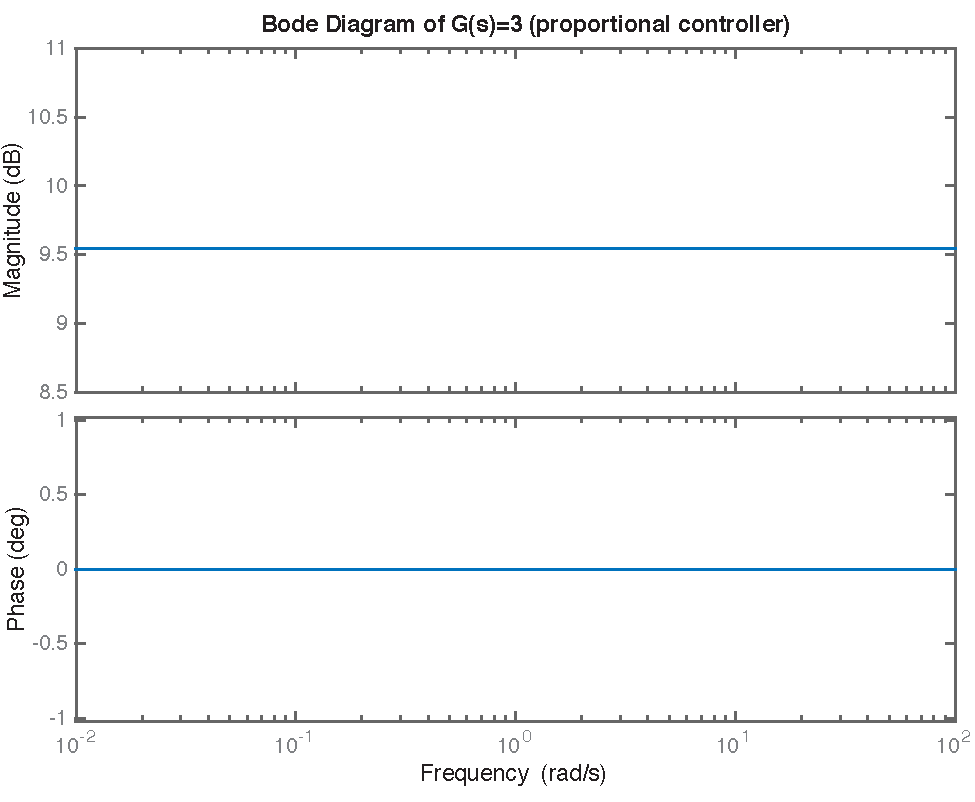
\includegraphics[width=.3\textwidth]{bodep.pdf}
}
\subfigure[Integral control]{
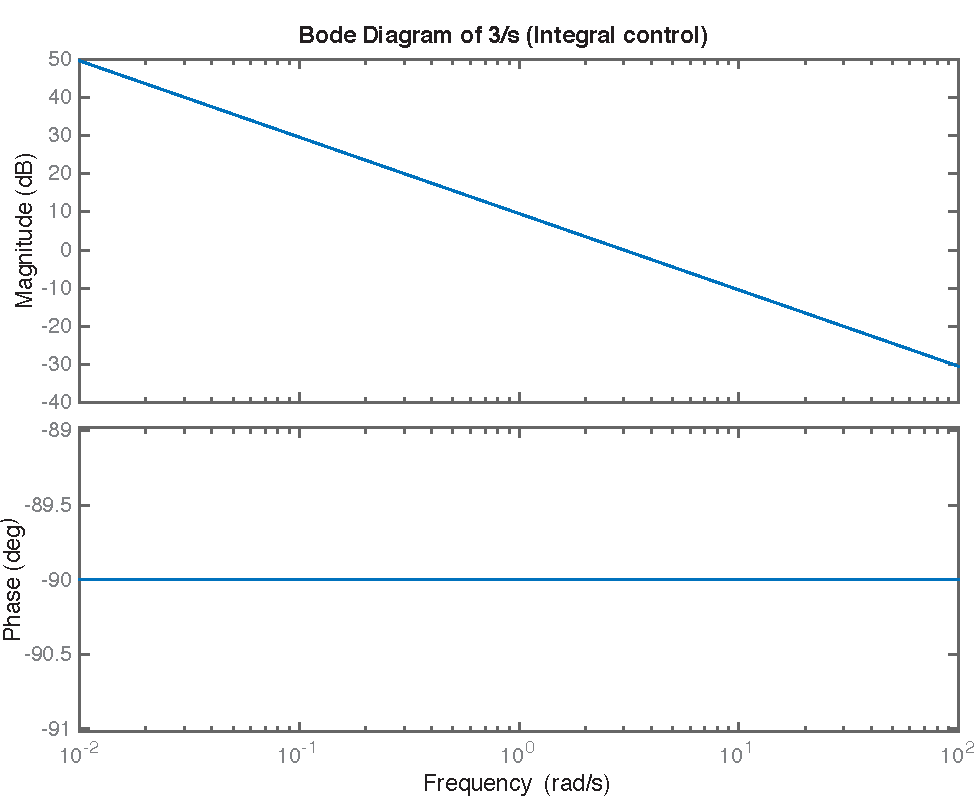
\includegraphics[width=.3\textwidth]{bodei.pdf}
}
\subfigure[Derivative control]{
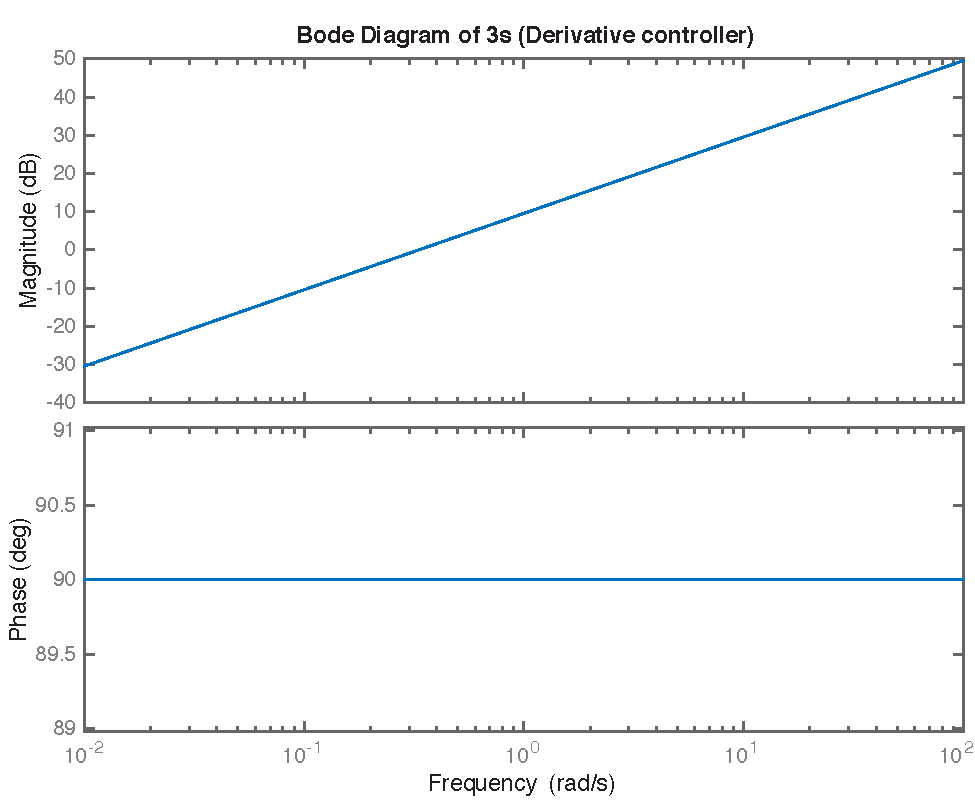
\includegraphics[width=.3\textwidth]{boded.pdf}
}
\label{fig:eachcomponentalone}
\end{figure}

\item High-pass: magnitude is high for high frequencies. Low-frequency: magnitude is high for low frequencies. Definition of bandwidth as range above -3 dB.

\item P-I controller:

\begin{eqnarray*}
G(s) & = & k +  \frac{1}{\tau_i s} = \frac{k\tau_i s + 1}{\tau_i s}\\ 
G(i\omega) & = &  \frac{k\tau_i \omega - i}{\tau_i \omega}\\
\left| G(i\omega) \right| & = & \sqrt{k^2 + \frac{1}{\tau_i^2 \omega^2} }\\
\phi &= &  \tan^{-1} \left( - \frac{1}{k \tau_i \omega} \right)
\end{eqnarray*}

Phase goes from -90 degrees to zero degrees; magnitude starts high and falls to around $k$ by $\omega \approx 1/\tau_i$ (the ``corner" or ``break" frequency).

\item P-D controller:

\begin{eqnarray*}
G(s) & = & k +  \tau_d s\\
G(i\omega) & = &  k + i \tau_d \omega\\
\left| G(i\omega) \right| & = & \sqrt{k^2 + \tau_d^2 \omega^2}\\
\phi &= &  \tan^{-1} \left( \frac{\tau_d \omega}{k} \right)
\end{eqnarray*}

Phase goes from zero degrees to ninety degrees; magnitude high and falls to around $k$ by $\omega \approx 1/\tau_i$ (the ``corner" or ``break" frequency).

\item A combination of proportional, integral, and derivative control can create a band stop filter:

\begin{eqnarray*}
G(s) & = & k + \tau_d s + \frac{1}{\tau_i s} = \frac{k\tau_i s + \tau_d \tau_i s^2 + 1}{\tau_i s}\\ 
G(i\omega) & = &\frac{1}{\tau_i \omega} \left( k \tau_i \omega +  i \left[ \tau_d \tau_i \omega^2 - 1 \right]  \right)\\
\left| G(i\omega) \right| & = & \sqrt{k^2 + \left( \tau_d \omega - \frac{1}{\tau_i \omega} \right)^2}\\
\phi &= & \tan^{-1}  \left( \frac{\tau_d \omega}{k} - \frac{1}{k\tau_i \omega} \right)
\end{eqnarray*}

The phase goes from -90 at small $\omega$ to +90 at high $\omega$.

\begin{figure}
\centering
\subfigure[PI control]{
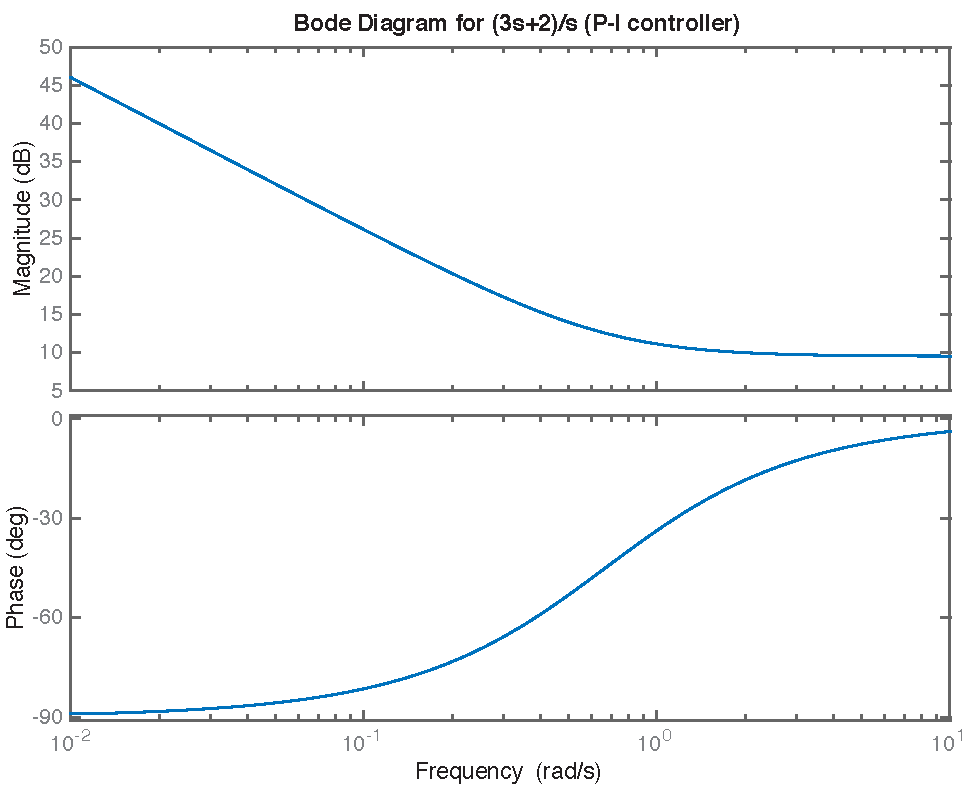
\includegraphics[width=.3\textwidth]{bodepi.pdf}
}
\subfigure[PD control]{
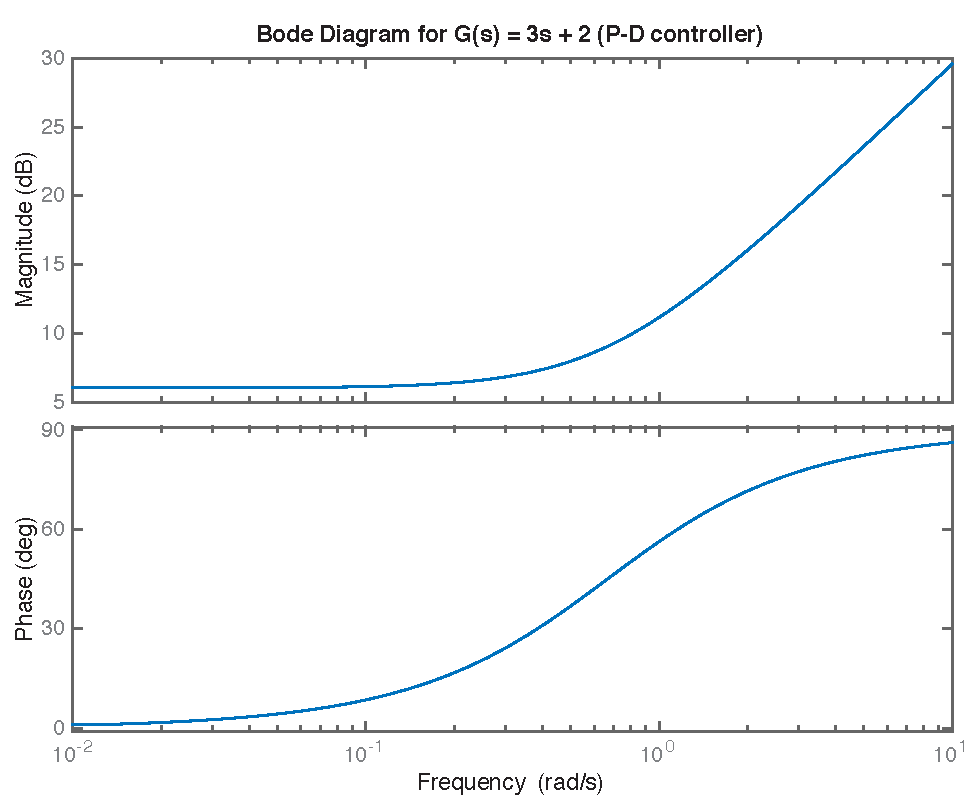
\includegraphics[width=.3\textwidth]{bodepd.pdf}
}
\subfigure[PID control]{
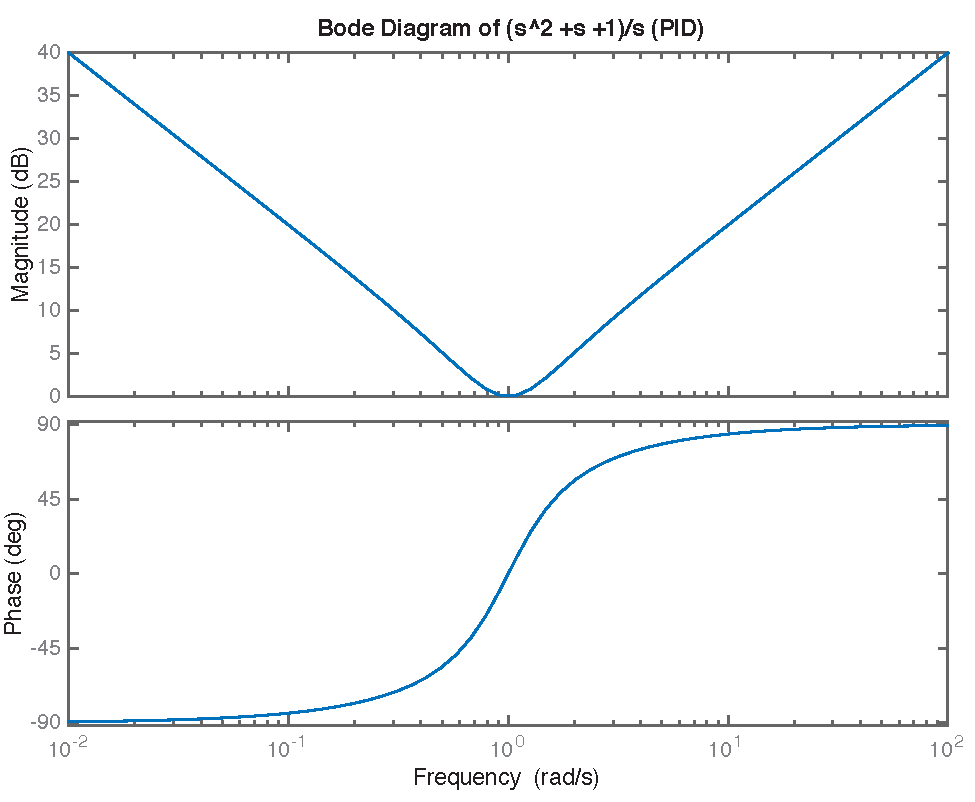
\includegraphics[width=.3\textwidth]{bodepid.pdf}
}
\label{fig:eachcomponentalone}
\end{figure}

\item Concept of lead-lag compensation -- not aware whether anyone has built or is looking for these in biological systems.

\end{itemize}

\section*{Application: yeast osmolarity regulation}
\begin{itemize}
\item Osmolarity: concentration of all solutes in a mixture.
\item When water is allowed to flow between two solutions (e.g. between cytoplasm and extracellular fluid through aquaporins), it will tend to move toward the region with more solutes.
\item An increased osmolarity outside the cell could draw out water, so in such media, yeast make more intracellular solutes until the osmolarity is sufficiently balanced.
\item Specifically, they make the small molecule glycerol under these hyper-osmotic conditions: we therefore call this response system the HOG pathway.
\item Diagram of the pathway simplifying figure 1 of Hershen et al., 2008.
\item In 2008 the Ramanathan lab constructed the moral equivalent of a Bode plot for the budding yeast HOG pathway.  They placed cells in a flow chamber and varied the osmolarity of the media in a square wave pattern of varying pulse length.
\item The output of the pathway was monitored by looking for nuclear entry of HOG1, a transcription factor mediating the response.
\item (Show frequency response analysis results.) What types of control does this pathway seem to display? What is the bandwidth of the pathway? 
\end{itemize}


\section*{Introduction to bacterial chemotaxis}

\begin{itemize}
\item Chemotaxis is movement towards a higher concentration of an attractant (or a lower concentration of a repellent).
\item The bacterium \textit{E. coli} swims forward when its many flagella all turn in the same direction (counter-clockwise).
\item  When one or more of the flagella rotate in the opposite direction,  it ``tumbles," splaying out its flagella and ceasing any relative motion. When the concentration of the attractant is spatially homogeneous, tumbling occurs about once per second.
\item During the tumble, the cell's direction is randomized. Eventually the errant flagellum will return to CCW spinning, and the cell begins to swim again, in a new direction.
\item \textit{E. coli} cannot steer, but they can still move in a particular direction on the net by controlling their tumbling rate. They tumble more often when they sense they're headed the ``wrong way," and vice versa.
\item In chemotaxis, the ``right way" is the direction in which the concentration of an attractant like leucine is increasing. \textit{E. coli} sense concentration using cell surface receptors. The fraction of receptors bound at any given time is a function of the ligand concentration (sketch a binding curve).
\item Suppose an \textit{E. coli} cell could detect the fraction of receptors bound at the front end, and compare it to the fraction of receptors bound at the back. Theoretically the cell would know if it were headed in the right direction. Unfortunately, this strategy does not work for \textit{E. coli} because of the small and finite number of receptors.
\item To grasp the problem, imagine a cell with only two receptors: one in front and one in back. The binding state at any instant would be too noisy to tell where [ligand] was higher, but the longer we wait, the more accurately we can measure the fraction of time that each receptor was occupied by ligand. The problem is that because \textit{E. coli} is so small, the concentration difference between the front and back of the cell must be small, so we would need to wait a very long time. Meanwhile the cell is swimming, changing direction etc.
\item Instead of comparing the concentrations at each end, the cell compares the current fraction of bound receptors to the fraction of bound receptors in the recent past (integrated over about the last four seconds). This timescale is appropriate because it balances the increased accuracy in $f_{\textrm{bound}}$ determination from long integration times with the fact that the cell doesn't tend to be going the same direction for very long. (Even when the cell does not tumble, it does not really swim straight: after four seconds it typically has changed orientation by about sixty degrees.)
\end{itemize}

\section*{Perfect adaptation in chemotaxis}

\begin{itemize}
\item You might expect that an \textit{E. coli} cell at steady-state in 0 nM ligand would tumble much more frequently than one at steady-state in a high ligand concentration.
\item In fact, the tumbling frequency at steady state is always the same: we say that tumbling frequency  \textit{adapts perfectly}.
\item This feature is very useful for ensuring that chemotaxis remains effective as a cell climbs a gradient, so that it can find more and more suitable environments.
\item You may already recognize the benefit of integral control in this system. But how, at a biochemical level, is it implemented?
\end{itemize}

\section*{The biochemical pathway and two models}

\begin{itemize}
\item The central player in the pathway is the receptor complex that binds extracellular attractants and regulates the intracellular response. We will call this receptor complex $E$\footnote{This notation does not match Alon but rather follows the original Barkai and Leibler paper.}.
\item $E$ can be bound or unbound by attractant ($E^b$ or $E^u$), and can be methylated or unmethylated ($E_0$ or $E_m$). All four variants are possible and we will refer to some subgroups of variants using a combination of these super- and subscripts.

\begin{center}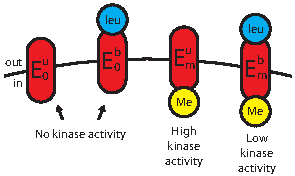
\includegraphics[width=.5\textwidth]{receptornotation.pdf}\end{center}

\item $E$ is methylated by an enzyme called CheR, which we will assume converts $E_0$ to $E_m$ at a constant rate independent of whether ligand is bound. This constant rate is realistic if $E_0$ always remains abundant enough that we stay in the right tail of CheR's Michaelis-Menten curve [draw this]. (Another way to phrase the assumption is that CheR is \textrm{operating at saturation}.)
\item Although $E$ can technically be methylated at multiple sites, for simplicity we will just assume that $E$ has one or zero methyl groups.

\begin{center}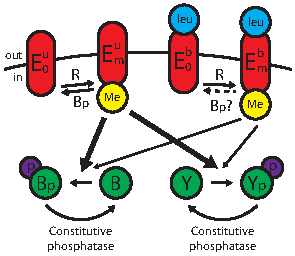
\includegraphics[width=.5\textwidth]{receptormethylation.pdf}\end{center}

\item The methylated form of $E$ is a kinase that can phosphorylate two downstream proteins, CheY and CheB. The \textit{activity} of the kinase is:

\[ A = \alpha_b E_m^b + \alpha_u E_m^u \]

That is, unmethylated receptors do not have any kinase activity. Unbound kinase is more active than bound kinase $(\alpha_u \gg \alpha_b)$.

\item CheY controls tumbling rate: as [CheY-P] increases, the tumbling frequency increases. (CheY-P is also converted back to CheY at a constitutive rate so it does not accumulate indefinitely.) When more ligand is added, $E$'s kinase activity decreases and CheY-P depletes, so less tumbling occurs, as you'd expect.

\item The other phosphorylation target of $E$ is its own demethylase, CheB. This is the crucial feedback loop that allows the circuit to adapt. Details on how CheB works is the only difference between the two models of perfect adaptation we will discuss today.

\item The steady-state tumbling rate depends on the steady-state concentration of CheY-P, which in turn depends on the steady-state activity of $E$ and CheY-P's dephosphorylation rate. Since the dephosphorylation rate is constant, we will have perfect adaptation (i.e. the steady-state tumbling rate will be the same at all ligand concentrations) if $A$ is independent of ligand concentration. We will try to determine when the latter condition holds.

\end{itemize}
\subsection*{Fine-tuned model}
\begin{itemize}
\item In the first model we will consider, phosphorylated CheB demethylates both $E_m^b$ and $E_m^u$ at the same rate. This means that we can write the total rate of change in $E_m$ as

\[ \frac{dE_m}{dt} = \frac{d \left(E_m^u + E_m^b \right)}{dt} = V_R - \frac{ V_{\textrm{max}} E_m}{K_m + E_m}  \]

where $V_R$ is the rate of CheR-mediated methylation (assumed to be saturated), and $V_{\textrm{max}}$ and $K_m$ are properties of CheB. $V_{\textrm{max}}$ is not really a constant, as it depends on the fraction of CheB that's phosphorylated.

\item The steady-state concentration of $E_m$ is

\[ 0 = \left. \frac{dE_m}{dt} \right|_{E_{\textrm{m, ss}}} \implies E_{\textrm{m,ss}} = \frac{V_R K_m}{V_{\textrm{max}} - V_R} \] 

\item When the concentration of attractant is zero, all of the $E_m$ is unbound, so at steady state:

\[ A_{\textrm{ss}} =  \alpha_b E_{\textrm{m,ss}}^b  + \alpha_u E_{\textrm{m,ss}}^u  = \alpha_u E_{\textrm{m,ss}} = \frac{ \alpha_u  V_R K_m}{V_{\textrm{max}}^1 - V_R} \]

The notation $V_{\textrm{max}}^1$ reminds us that the maximum rate of CheB depends on what fraction of it is phosphorylated.

\item On the other hand, when the concentration of attractant is saturating, all of the $E_m$ is bound and at steady-state:

\[ A_{\textrm{ss}} = \alpha_b E_{\textrm{m,ss}}^b + \alpha_u E_{\textrm{m,ss}}^u  = \alpha_b E_{\textrm{m,ss}} = \frac{ \alpha_b  V_R K_m}{V_{\textrm{max}}^2 - V_R} \]

Notice that the maximum rate of demethylation has changed because less of the demethylase [CheB-P] will be present at steady-state.

\item These two activities (and indeed, the activity at every intermediate ligand concentration) must be the same in order for the system to display perfect adaptation.

\item While hypothetically possible, this would require exquisite tuning of these parameters through evolution. A major concern is introduced by the variation in gene expression between cells.

\item It is quite common for protein concentrations to vary by, say, 20\% between cells. Uri Alon provides a numerical answer where a 20\% change in the concentration of one protein (CheR) leads to a three-fold change in activities between the two states -- nowhere close to perfect adaptation. (In fact the error could be much worse, depending on what the values for these parameters actually are.) We say that perfect adaptation is a fine-tuned property of this model.
\end{itemize}

\subsection*{A robust model for perfect adaptation} 
 
\begin{itemize} 
 
\item Barkai and Leibler (1997) provide a model for this system that is much more resilient to variation in gene expression and other parameters of the model. The only essential difference is that CheB-P can only demethylate $E_m^u$, so:

\[ \frac{dE_m}{dt} = \frac{d \left(E_m^u + E_m^b \right)}{dt} = V_R - \frac{ V_{\textrm{max}} E_m^u}{K_m + E_m^u}  \]

\item At steady state:

\[ 0 = \left. \frac{dE_m}{dt} \right|_{E_{m,\textrm{ss}}^u} \implies E_{m,\textrm{ss}}^u = \frac{V_R K_m}{V_{\textrm{max}} - V_R} \]

\item In other words, the receptor's kinase activity

\[ A =  \alpha_b E_m^b + \alpha_u E_m^u \approx \alpha_u E_m^u \]

always approaches the same steady-state value, regardless of ligant concentration. Consequently, [CheY-P] will approach the same steady state value as well. This is perfect adaptation.

\item This model makes essentially no requirements on the parameters (other than that our assumptions that CheR operates at saturation and $\alpha_u \gg \alpha_b$ stay valid). In other words, the construction of the pathway is all that is needed to implement the perfect adaptation.

\item Let's recap what is happening in this system. Suppose the cell has adapted to its media and we suddenly add more attractant.
\begin{itemize}
\item  The activity plummets immediately as $E_m^u$ converts to $E_m^b$.
\item This gives rise to a transient decrease in tumbling frequency.
\item Meanwhile, less CheB is phosphorylated than usual due to the low receptor kinase activity: the level of CheB-P begins to fall.
\item This shifts the balance toward methylation of $E$, creating more $E_m$ until the activity returns to its normal value.
\end{itemize}

\end{itemize}

\section*{Perfect adapation always requires integral control}

\begin{itemize}

\item Recall that proportional control results in \textit{droop} (non-zero error at steady-state) and that integral control provides a means to reduce the operating error to zero at steady-state. In control theory, this is called asymptotic tracking (which means the same thing as perfect adaptation).

\item This system implements integral control: the integration (memory of past ligand concentrations) is effected through accumulation or depletion of methyl groups. If the concentration was high recently, then there will be few methyl groups; if it was low recently, then there will be more methyl groups.

\item Control is then exerted by allowing the number of methyl groups to affect the activity of the receptor complex.

\item Your next discussion paper will be on another example of perfect adaptation: this time, in the yeast hyperosmotic glycerol (HOG) response.

\item We have seen an example of integral control applied in biology; on Monday, we'll look at a biological system effecting derivative control.

\end{itemize}

\end{document}